\documentclass[12pt]{article}

\usepackage{fontawesome}
\usepackage{hyperref}
\usepackage{xurl}
\usepackage{graphicx}



\hypersetup{
    colorlinks=false,
    pdfborder={0 0 0},
}


\title{SQL Continued}
\author{
        Adrianna Holden-Gouveia \\
        Website: \url{https://aholdengouveia.name}\\ 
        \date{\vspace{-5ex}}
        %Email: \href{mailto:admin@aholdengouveia.name}{admin@aholdengouveia.name} \\
        \faLinkedin{: aholdengouveia} \\
        \faGithub {: aholdengouveia} \\
        \faTwitter {: aholdengouveia} \\
        }

%S\date{\today}


\begin{document}    

\maketitle

%\begin{abstract}
%This is a template for Linux Administration Lab work
%\end{abstract}
%\tableofcontents

\section*{Objectives:}
\begin{itemize}
    \item The objective of this lab is to continue working with SQL to learn more advanced topics such as filters and functions. Prior knowledge SQL is assumed. Students will gain a understanding of SQL functions and filters through interactive methods utilizing a free online tutorial and other resources.
\end{itemize}
\section*{Instructions}

References, a video, a PowerPoint and some notes are available at my website
\url {https://www.aholdengouveia.name/IntroData/sql2.html}

The tutorial you will be following is here: \url{https://www.sqltutorial.org/} 
You will be doing the following sections of this tutorial.  You may do more if you want.
\begin{itemize}
    \item SELECT
    \item DISTINCT
    \item ORDER BY
    \item AND
    \item OR
    \item UPDATE
    \item INSERT
    \item DELETE
\end{itemize}

\subsection*{Please include answers to the following questions}
    \begin{enumerate}
        \item How do you think this compares to the first tutorial from  \url{https://selectstarsql.com/}?
        \item What do you think is missing from this tutorial? Why?
        \item What is a use case example for each of the 8 topics for your data?  For example, for books I might want to add a book, delete a book, or change an author.  
        \item Take screenshots of the question you found most challenging in each section (there should be 8 screenshots total), make sure to have a note with your name and the term in the screenshot, screenshot should be focused on the note and answer, not the full desktop.  Any screenshots that don't include the note, or are full desktop, or taken with a camera instead of a screenshot won't count and will earn no points. This is an example of what it should look like:        
 
        \begin{figure}[h!]
            \centerline{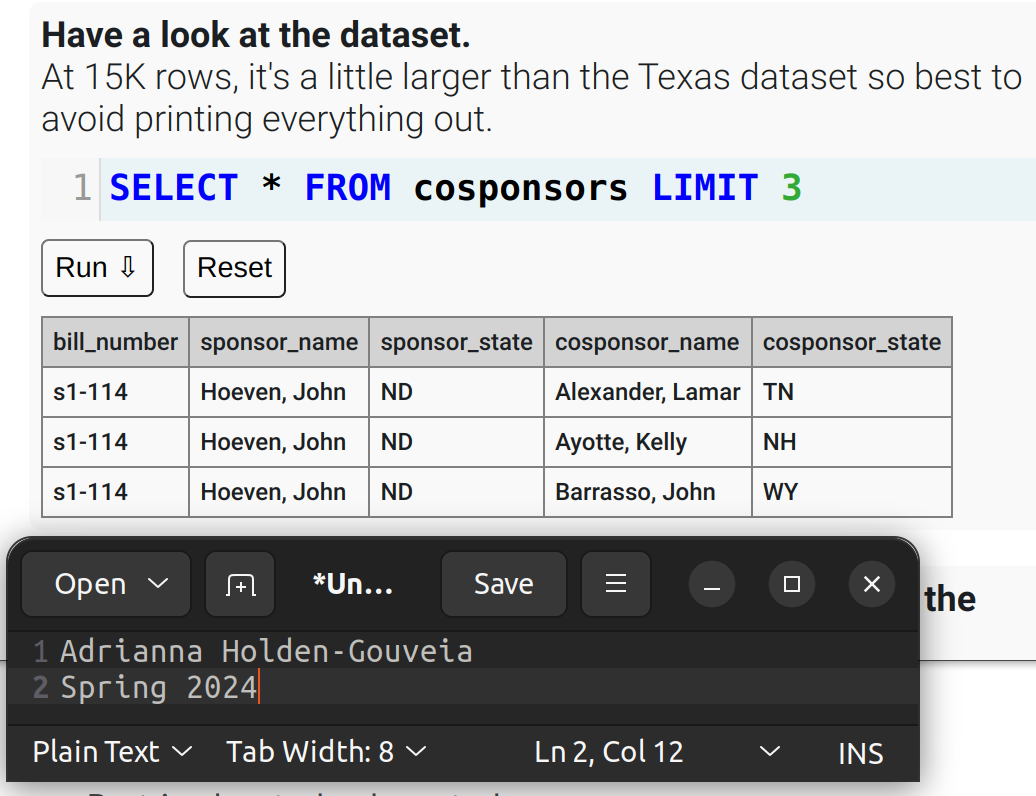
\includegraphics[scale=.2]{Examplewk6.png}}
            \caption{This is an image of what each of your screenshots should look like}

            \end{figure} 
    \end{enumerate}

    \section*{Tutorial Recommendation}
You should find a tutorial that you would recommend to another person that wanted to learn SQL filters and functions.  The tutorial can be interactive or not.  Videos that you can follow along with count as tutorials for this. You should find at least 3 options for tutorials/videos that you also include here. In your recommendation you should explain why you picked the one you did over the other two including pros and cons of each. You may not include any of the links I've shared in your list, they must be new to you materials and tutorials/videos. 


\section*{Deliverables}
\begin{itemize}
    \item A document containing all requested screenshots
    \item Answers to the above questions
    \item Your tutorial recommendation.  Review should be at least a paragraph but no more then two pages. 
\end{itemize} 
\end{document}